% !Mode:: "TeX:UTF-8"
\documentclass[a4paper, 11pt]{article}
\usepackage{xeCJK}
\setCJKmainfont{AR PL UMing CN} 
\usepackage{comment} % enables the use of multi-line comments (\ifx \fi)
\usepackage{lipsum} %This package just generates Lorem Ipsum filler text.
\usepackage{fullpage} % changes the margin
\usepackage{hyperref}

\begin{document}
%Header-Make sure you update this information!!!!
\noindent

\large\textbf{Conclusion Report}
\hfill \textbf{Exchange Simulator Project / Team B} \\

\normalsize Course code: CS28011 \hfill Prof. Jian Cao \& Dr. James L. Mei\\

TA: Nengjun Zhu  \hfill Due Date: 2016/12/30 \\

Teammates:
%TODO all write your student number, check your name
Alexander Goscinski 116030990050

Ruth-Emely Pierau 116030990078

Valentin Rothoft
 %TODO valentin 

Yelinsheng(查汗巴依尔·叶林生) 116033910057

Husein Sulianto 116030990100



\section*{System Architecture}

\section*{Key Techniques}

The project is mainly written in python. We used python 2.7. For some features like the matching algorithm the numpy library \cite{numpy} was used.
For the FIX communication we used the quickfix library. For the database we use MySQL and use the library MySQL-python as interface between python and MySQL.
\subsection*{Order Matching}

%TODO Valentin
\subsection*{FIX}
QuickFIX library is an Open Source FIX engine library, it support several programming language C++,Python,Ruby,Java and .NET. 
In the current project, we use QuickFIX library version 1.14.3 (current latest version). QuickFix provide throughout fix message definition for every message which can be configured for each the project.
It also support mandatory field checking for each type of message.
\subsection*{Database}

For the database MySQL 5.7.15 was used. We created the diagrams and sql scripts creating the structure of the database with MySQL Workbench.
As interface between python any MySQL we used MySQL-python version 1.2.5.
\subsubsection*{Server}
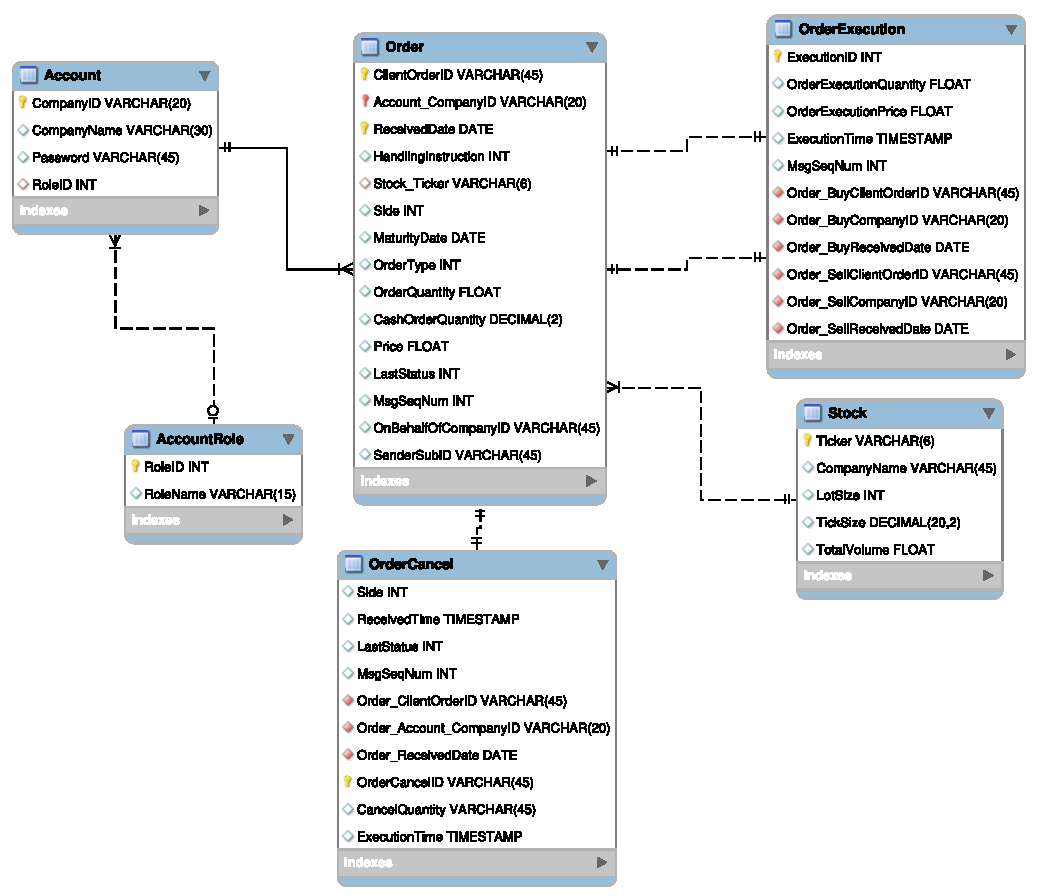
\includegraphics{../diagrams/server_database.pdf}

\paragraph*{Account}
Table to store user account is allowed to connect to the server
\textbf{CompanyID:} the ID of the company when the company registered
\textbf{CompanyName:} The name of the company with given companyID
\textbf{Password:}The password of the company
\textbf{RoleID:}The role of the user, if he is has admin rights (1) or no admin rights (0)

\paragraph*{Order}
Table to store order sent by client to buy or sell stocks.
\textbf{ClientOrderID:}The Order ID sent by the client 
\textbf{Account_CompanyID:}The ID of the company making the order
\textbf{ReceivedDate:}The date when the order was first accepted
\textbf{HandlingInstruction:}The way the order should be handled (supported values 1 = Automated execution order, private, no Broker intervention)
\textbf{Stock_Ticker:}The ticker symbol of the requested order
\textbf{Side:}The side of an Order (1: Buy, 2: Sell)
\textbf{OrderType:}The type of order (1: Market , 2: Limit)
\textbf{OrderQuantity:} The total quantity of the order (be careful, it could be that the order is partially fulfilled, therefore it has to be checked if there exist
\textbf{CashOrderQuantity:}The cash amount to represent the order for client (given the cash amount quantity of order will be computed separately) (is not supported)
\textbf{Price:}The price of orderrequested by client
\textbf{LastStatus:}The current status of order in server side(0:Done, 1:Pending, 2: Canceled, 3:Expired)
\textbf{MsqSeqNum:}Message Sequence Number of Order sent by client, stored in case of robustness data needed
\textbf{OnBehalfOfCompanyID:}The original sender of the order therefore if filled the current order is sent by intermediary to server 
\textbf{SenderSubID	:}The additional information of sender given by client

\paragraph*{OrderCancel}
Table to store order cancel sent by client
\textbf{Side}The side of an Order to be cancelled (1: Buy, 2: Sell)
\textbf{ReceivedTime}The time when the order cancel was first accepted by server
\textbf{LastStatus}The current status of order cancel in server side(1:Pending, 2: Canceled)
\textbf{MsgSeqNum}Message Sequence Number of Order Cancel sent by client, stored in case of robustness data needed
\textbf{Order_ClientOrderID}Represent The Order ID need to be cancelled by the client (same as OrigClientOrderID in FIX Cancel Order request)
\textbf{Order_Account_CompanyID}The ID of the company making the order (same with ID of company making order cancel)
\textbf{Order_ReceivedDate}The date when the order was first accepted
\textbf{OrderCancelID}Represent the Order Cancel ID sent by client (same as OrderID in FIX Cancel Order request)
\textbf{CancelQuantity}The total amount of quantity which is cancelled related to the order
\textbf{ExecutionTime}The time when the order cancel was executed by server
   
\paragraph*{Stock}
Table to store information of trading stock supported by server
\textbf{Ticker:}Stock Symbol represent the commodity/company in the market
\textbf{CompanyName:}Increment quantity for buying/selling stock
\textbf{LotSize:}The name of the company with given stock symbol
\textbf{TickSize:}minimum price movement of a trading instrument
\textbf{TotalVolume:}Total number of shares for the stock
 	 
\paragraph*{OrderExecution}
Table to store executed/matched order including buying side and selling side
\textbf{ExecutionID:}ID of executed order transaction generated by server
\textbf{OrderExecutionQuantity:}Quantity of order in sell/buy side which is matched
\textbf{OrderExecutionPrice:}Price of order in sell/buy side matched
\textbf{ExecutionTime:}The time order executed is done
\textbf{MsgSeqNum:}Message Sequence Number of Order Execution sent by server, stored in case of robustness data needed	
\textbf{Order_BuyClientOrderID:}The buyer Order ID sent by the client 
\textbf{Order_BuyCompanyID :}The buyer Company ID making the order	
\textbf{Order_BuyReceivedDateThe:}Date when the order sent by buyer 
\textbf{Order_SellClientOrderID:}The seller Order ID sent by the client
\textbf{Order_SellompanyID:}The seller Company ID making the order
\textbf{Order_SellReceivedDate:}Date when the order sent by seller 

\subsubsection*{Client}
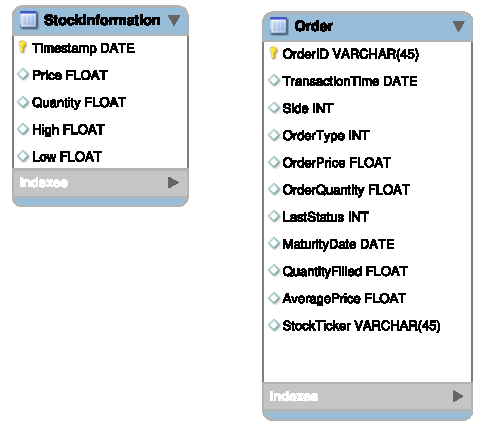
\includegraphics{../diagrams/client_database.pdf}
\paragraph*{StockInformation}
Table to store stock price and quantity at given time
\textbf{Timestamp:}The date stock information is published
\textbf{Price:}The price of the stock at given timestamp 
\textbf{Quantity:}The quantity of stock at given timestamp 
\textbf{High:}The highest price value of stock at given timestamp
\textbf{Low:}The lowest price value of stock at given timestamp

\paragraph*{Order}
Table to store order created by client ,it record the progress and status of order
\textbf{OrderID:}The id of an order from client side. In the FIX protocol this is named as ClientOrderID.
\textbf{TransactionTime:}The time client sent order to server 
\textbf{Side:}The side of Order (1: Buy, 2: Sell)
\textbf{OrderType:}The type of Order (1: Market , 2: Limit)
\textbf{OrderPrice:}The price of the order for one Lot size (for now standard lotsize is everywhere 1)
\textbf{OrderQuantity:}The quantity of an order
\textbf{LastStatus:}The current status of order in client side (0:DONE, 1:PENDING, 2: CANCELED, 3:EXPIRED, 4: NOT_YET_ACKNOWLEDGED, 5:REJECTED)
\textbf{MaturityDate:}Final payment date for financial instrument type stock
\textbf{QuantitiyFilled:}The quantity of this order which has been already filled agains the opposite side order
\textbf{AveragePrice:}The average price the order was sold. This field is 0, if quantity has  not been sold.
\textbf{StockTicker:} Stock Symbol represent the commodity/company in the market

\subsection*{GUI}
\begin{itemize}
  \item Use python's GUI library HtmlPy to create GUI using html, css, javascript.
  \item Use CSS library Bootstrap to create fancy front end page. 
  \item Use JS library Jquery to add logic.
\end{itemize}




\section*{Task Allocation Among Members}

Alexander Goscinski:
\begin{itemize}
  \item Implementation and maintenance of system architecture
  \item Manage tasks
\end{itemize}
Ruth-Emely Pierau:
\begin{itemize}
	\item Implementation and testing of Matching Algorithm
	\item Implementation of some functions for testing server logic
	\item Implementation of some basic data classes
\end{itemize}
Yelinsheng(查汗巴依尔·叶林生):
\begin{itemize}
  \item GUI implementation
  \item Some functions of client logic
  \item Some functions of server logic
  \item Implementation of some basic data classes
  \item Code testing
\end{itemize}
Husein Sulianto:
\begin{itemize}
  \item Designing overview of Database
  \item Do Order Canceling function in client and server side
  \item Implementation of several basic data classes and fix message definition layout
  \item Code testing
\end{itemize}
Valentin
%TODO Valentin

% to comment sections out, use the command \ifx and \fi. Use this technique when writing your pre lab. For example, to comment something out I would do:
%  \ifx
%   \begin{itemize}
%       \item item1
%       \item item2
%   \end{itemize}
%  \fi

\section*{Workload Allocations}
Total 100\% \\

\section*{Other}
\lipsum[7]

\section*{Conclusion}
The usage of the quickfix library with pythos is recommended because the port is not fitted to python code. It is mostly Java code with python grabbers.

\section*{Attachments}
Project homepage with installation instructions: \url{https://github.com/agoscinski/fsc} \\
Demo video (password: sjtu1896): \url{https://owncloud.tu-berlin.de/index.php/s/ihEUWxj8FvIAZhI}

\begin{thebibliography}{9}
\bibitem{numpy} Developers, NumPy. "NumPy." NumPy Numpy. Scipy Developers (2013) \url{https://docs.scipy.org/doc/numpy-dev/numpy-ref.pdf}.
\end{thebibliography}

\end{document}
